Ниже приведены графики, полученные в результате работы реализованной программы.

\begin{figure}[H]
	\begin{center}
		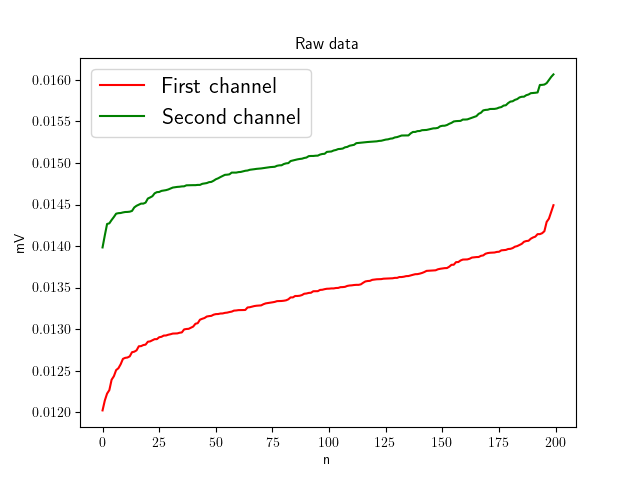
\includegraphics[scale=0.78]{rawdata}
		\label{pic:rawdata}
		\caption{Загруженные данные}
	\end{center}
\end{figure}

\begin{figure}[H]
	\begin{center}
		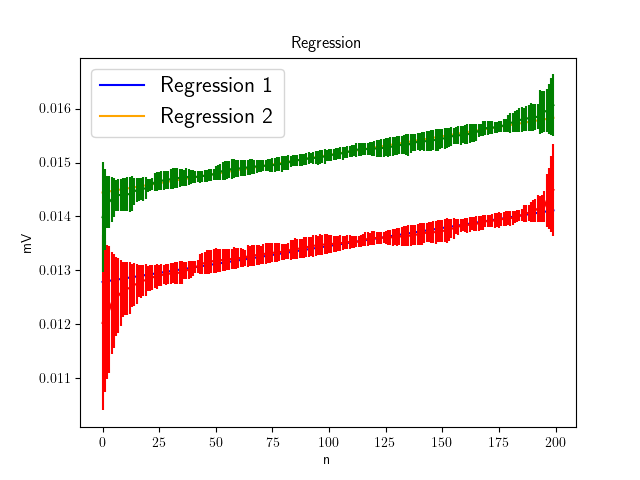
\includegraphics[scale=0.68]{regression}
		\label{pic:regression}
		\caption{Линейная регрессия для вещественных данных и результаты обынтерваливания}
	\end{center}
\end{figure}

\begin{table}[H]
	\begin{center}
		\begin{tabular}{|c|c|c|}
			\hline
			N & $\beta_0$ & $\beta_1$ \\
			\hline
			1 & 0.012 & 6.67e-6 \\
			\hline
			2 & 0.014 & 6.96e-6 \\
			\hline
		\end{tabular}
		\caption{Параметры линейной регрессии для двух входных наборов данных}
	\end{center}
\end{table}

\begin{figure}[H]
	\begin{center}
		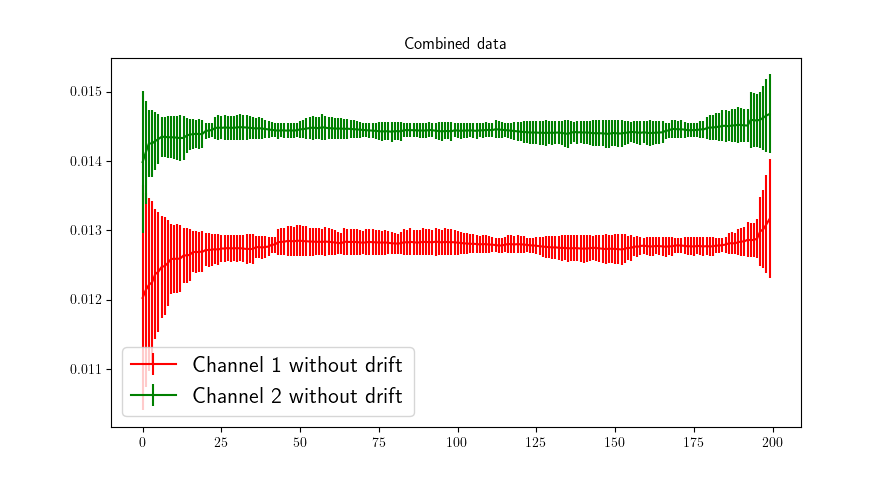
\includegraphics[scale=0.85]{horizontal}
		\label{pic:horizontal}
		\caption{Данные после вычитания ``наклонной'' составляющей}
	\end{center}
\end{figure}

\begin{figure}[H]
	\begin{center}
		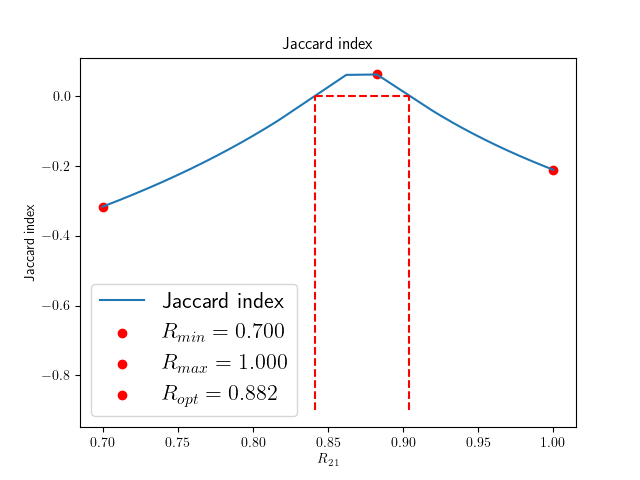
\includegraphics[scale=0.85]{jaccard}
		\label{pic:jaccard}
		\caption{Зависимость коэффициента Жаккара от $R_{21}$}
	\end{center}
\end{figure}

Оптимальное соотношение $R_{opt} = 0.885$, было найдено в диапазоне $[0.774; 0.953]$.

\begin{figure}[H]
	\begin{center}
		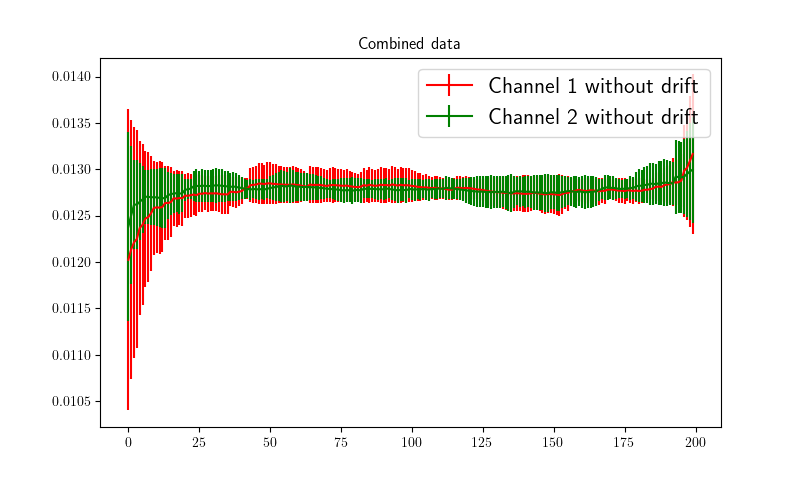
\includegraphics[scale=0.85]{result}
		\label{pic:result}
		\caption{Результат наложения данных при максимальном коэффициенте Жаккарда}
	\end{center}
\end{figure}
